\documentclass[conference]{IEEEtran}

\usepackage{booktabs}
\usepackage{amsmath}
\usepackage{bm}
\usepackage{tikz}
\usetikzlibrary{arrows,shadows} % for pgf-umlsd
\usepackage[underline=true,rounded corners=false]{pgf-umlsd}

\newcommand{\hy}{\hbox{-}\nobreak\hskip0pt}

\newcommand{\NP}{\text{\normalfont NP}}

\usepackage{hyperref}

\begin{document}
	
% paper title
\title{Improving Directed Ramsey Numbers using SAT}

\author{\IEEEauthorblockN{David Neiman, Marijn Heule, and John Mackey}
\IEEEauthorblockA{Carnegie Mellon University, Pittsburgh, United States}

}


\newcommand{\mc}{}

\maketitle

\section*{Intro}

%The suite consists of miters: equivalence checking problems of 
%Boolean circuits. 

A tournament is an orientation of a complete graph, or equivalently a directed graph $D$ 
with no self-loops such that, for all pairs of distinct vertices $u$ and $v$, exactly one of
the edges $uv$ or $vu$ is in $D$. Intuitively, a tournament of order $n$ represents the
results of a round-robin tournament between $n$ teams, where the existence of edge
$uv$ means team $u$ beat team $v$ in their head-to-head match. The exclusivity of
$uv$ and $vu$ means that if team $u$ beats team $v$, team $v$ doesn't beat team
$u$, and the inclusion of one of those edges reflects the fact that in a round-robin
tournament, each team plays each other team. The non-existence of self-loops translates to the fact that no team plays itself.

A tournament is \textit{transitive} if, for all vertices $a$, $b$, and $c$, the existence of edges $ab$ and $bc$ implies the existence of edge $bc$.
If a tournament is not transitive, then it contains a directed cycle of length 3.


\begin{figure}[ht]
\centering
  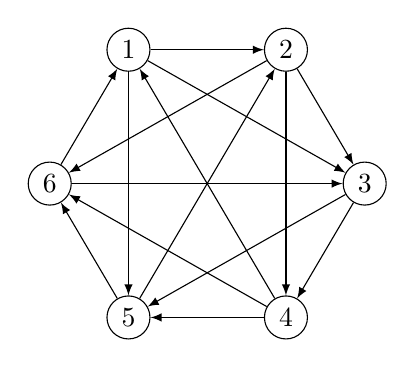
\begin{tikzpicture}
    \node[circle, draw] (1) at (0,0) {\!1\!};
    \node[circle, draw] (2) at (2,0) {\!2\!};
    \node[circle, draw] (3) at (3,-1.7) {\!3\!};
    \node[circle, draw] (4) at (2,-3.4) {\!4\!};
    \node[circle, draw] (5) at (0,-3.4) {\!5\!};
    \node[circle, draw] (6) at (-1,-1.7) {\!6\!};
    
    \draw (1) edge[-latex] (2) (1) edge[-latex]  (3) (1) edge[-latex]  (5) (4) edge[-latex] (1) (6) edge[-latex]  (1);
    \draw (2) edge[-latex] (3) (2) edge[-latex]  (4) (2) edge[-latex]  (6) (5) edge[-latex] (2) (3) edge[-latex]  (4);
    \draw (3) edge[-latex] (5) (6) edge[-latex]  (3) (4) edge[-latex]  (5) (4) edge[-latex] (6) (5) edge[-latex]  (6);

  \end{tikzpicture}
\caption{The unique tournament of order 6 without a transitive sub-tournament of order 4.}
\end{figure}


\section*{Directed Ramsey Numbers}
The directed Ramsey number $R(k)$ is the smallest integer $n$ such that all
tournaments on $n$ vertices contain a transitive tournament of order  $k$.

Directed Ramsey numbers were first introduced by Erd\H{o}s and Moser~\cite{ErdosMoser}. 
In particular, they showed that $k \leq 2 \log_2(R(k)) + 1$ and also noted that $k \geq \log_2(R(k)) + 1$. 
In particular, this means $R(k)$ grows roughly as an exponential of $k$, with multiplier somewhere
between $\sqrt{2}$ and 2. The precise limit of that multiplier is not known, but the literature has the following
results on small directed Ramsey numbers:

\begin{itemize}
\item $R(2) = 2$
\item $R(3) = 4$
\item $R(4) = 8$
\item $R(5) = 14$
\item $R(6) = 28$ (\cite{SanchezFlores55})
\item $32 \leq R(7) \leq 54$ (\cite{SanchezFlores54})
\end{itemize}

The tournaments of order 25, 26, and 27 that do not contain a 
transitive sub-tournament of order 6 are unique. We call them $ST_{25}$,
$ST_{26}$, and $ST_{27}$, respectively. There are five 
tournaments of order 24 without a transitive sub-tournament of order 6.



\section*{SAT Encoding}

Lower bounds of directed Ramsey number $R(k)$ can be improved by 
constructing a complete directed graph without a transitive tournament
of order $k$. The direct encoding into SAT would only use boolean 
variables for each edge with the truth value of a variable denoting 
the direction of the edge. Such an encoding uses many clauses and
the resulting formulas are too large to improve the lower bound of
$R(7)$. We therefore constructed a more compact encoding, which
uses the fact that a transitive tournament lacks a directed cycle of
length 3. For each triple of vertices in the graph, we introduce 
a new variable that is true if and only if the edges between them 
form a directed cycle. We use these auxiliary variables to encode 
the absence of transitive tournaments of order $7$ more 
compactly.

\section*{Benchmarks}

We submitted 16 benchmarks to the 2020 SAT Competition. The first
8 formulas encode whether $ST_{25}$, $ST_{26}$, $ST_{27}$, and the five
tournaments of order 24 without a transitive sub-tournament of order 6
can be extended to a tournament of order 33 without creating a
transitive sub-tournament of order 7. All these instances are satisfiable
and thus establish an improved lower bound $R(7) > 33$. Figure~\ref{fig:lowerbound} shows an example. The second 8
formulas are similar, but encode the existence of a tournament of order 34
without creating a transitive sub-tournament of order 7. It is not known 
whether these instances are satisfiable.


\newcommand*\circled[1]{\tikz[baseline=(char.base)]{
            \node[fill=black,shape=circle,draw,inner sep=1pt] (char) {\textcolor{white}{#1}};}}

\newcommand{\zero}{0}
\newcommand{\one}{\circled{1}}

\begin{figure*}[ht]
\begin{center}

\begin{tabular}{c@{\,}c@{\,}c@{\,}c@{\,}c@{\,}c@{\,}c@{\,}c@{\,}c@{\,}c@{\,}c@{\,}c@{\,}c@{\,}c@{\,}c@{\,}c@{\,}c@{\,}c@{\,}c@{\,}c@{\,}c@{\,}c@{\,}c@{\,}c@{\,}c@{\,}c@{\,}c@{\,}c@{\,}c@{\,}c@{\,}c@{\,}c@{\,}c}
\zero& \one& \one& \one& \one& \zero& \one& \zero& \zero& \one& \one& \zero& \one& \one& \zero& \zero& \zero& \one& \one& \zero& \zero& \zero& \zero& \one& \zero& \one& \zero& \one& \zero& \zero& \zero& \one& \one\\
\zero& \zero& \zero& \zero& \zero& \zero& \one& \zero& \one& \one& \zero& \zero& \one& \zero& \zero& \one& \one& \one& \zero& \zero& \one& \one& \one& \one& \zero& \one& \one& \zero& \one& \zero& \zero& \one& \one\\
\zero& \one& \zero& \one& \one& \one& \one& \zero& \one& \zero& \zero& \one& \one& \zero& \one& \one& \zero& \zero& \zero& \one& \one& \zero& \zero& \zero& \zero& \one& \zero& \one& \zero& \zero& \one& \one& \zero\\
\zero& \one& \zero& \zero& \zero& \zero& \zero& \zero& \one& \zero& \one& \one& \zero& \zero& \one& \zero& \zero& \one& \one& \one& \zero& \zero& \one& \one& \one& \one& \one& \zero& \one& \one& \zero& \zero& \one\\
\zero& \one& \zero& \one& \zero& \one& \one& \one& \one& \zero& \one& \zero& \zero& \one& \one& \zero& \one& \one& \zero& \zero& \zero& \one& \one& \zero& \zero& \zero& \zero& \one& \zero& \zero& \one& \zero& \one\\
\one& \one& \zero& \one& \zero& \zero& \zero& \zero& \zero& \zero& \one& \zero& \one& \one& \zero& \zero& \one& \zero& \zero& \one& \one& \one& \zero& \zero& \one& \one& \one& \one& \zero& \one& \zero& \one& \zero\\
\zero& \zero& \zero& \one& \zero& \one& \zero& \one& \one& \one& \one& \zero& \one& \zero& \zero& \one& \one& \zero& \one& \one& \zero& \zero& \zero& \one& \one& \zero& \zero& \one& \zero& \one& \one& \zero& \zero\\
\one& \one& \one& \one& \zero& \one& \zero& \zero& \zero& \zero& \zero& \zero& \one& \zero& \one& \one& \zero& \zero& \one& \zero& \zero& \one& \one& \one& \zero& \zero& \one& \one& \one& \zero& \one& \zero& \zero\\
\one& \zero& \zero& \zero& \zero& \one& \zero& \one& \zero& \one& \one& \one& \one& \zero& \one& \zero& \zero& \one& \one& \zero& \one& \one& \zero& \zero& \zero& \one& \zero& \zero& \zero& \zero& \one& \one& \one\\
\zero& \zero& \one& \one& \one& \one& \zero& \one& \zero& \zero& \zero& \zero& \zero& \zero& \one& \zero& \one& \one& \zero& \zero& \one& \zero& \zero& \one& \one& \one& \one& \one& \zero& \one& \one& \one& \one\\
\zero& \one& \one& \zero& \zero& \zero& \zero& \one& \zero& \one& \zero& \one& \one& \one& \one& \zero& \one& \zero& \zero& \one& \one& \zero& \one& \one& \zero& \zero& \zero& \one& \zero& \zero& \zero& \zero& \zero\\
\one& \one& \zero& \zero& \one& \one& \one& \one& \zero& \one& \zero& \zero& \zero& \zero& \zero& \zero& \one& \zero& \one& \one& \zero& \zero& \one& \zero& \zero& \one& \one& \zero& \one& \zero& \one& \one& \zero\\
\zero& \zero& \zero& \one& \one& \zero& \zero& \zero& \zero& \one& \zero& \one& \zero& \one& \one& \one& \one& \zero& \one& \zero& \zero& \one& \one& \zero& \one& \one& \zero& \one& \zero& \one& \zero& \one& \zero\\
\zero& \one& \one& \one& \zero& \zero& \one& \one& \one& \one& \zero& \one& \zero& \zero& \zero& \zero& \zero& \zero& \one& \zero& \one& \one& \zero& \zero& \one& \zero& \one& \one& \one& \one& \zero& \zero& \zero\\
\one& \one& \zero& \zero& \zero& \one& \one& \zero& \zero& \zero& \zero& \one& \zero& \one& \zero& \one& \one& \one& \one& \zero& \one& \zero& \zero& \one& \one& \zero& \zero& \zero& \zero& \one& \one& \zero& \one\\
\one& \zero& \zero& \one& \one& \one& \zero& \zero& \one& \one& \one& \one& \zero& \one& \zero& \zero& \zero& \zero& \zero& \zero& \one& \zero& \one& \one& \zero& \zero& \one& \one& \one& \zero& \one& \zero& \zero\\
\one& \zero& \one& \one& \zero& \zero& \zero& \one& \one& \zero& \zero& \zero& \zero& \one& \zero& \one& \zero& \one& \one& \one& \one& \zero& \one& \zero& \zero& \one& \zero& \one& \zero& \zero& \zero& \one& \one\\
\zero& \zero& \one& \zero& \zero& \one& \one& \one& \zero& \zero& \one& \one& \one& \one& \zero& \one& \zero& \zero& \zero& \zero& \zero& \zero& \one& \zero& \one& \one& \one& \zero& \one& \zero& \one& \one& \zero\\
\zero& \one& \one& \zero& \one& \one& \zero& \zero& \zero& \one& \one& \zero& \zero& \zero& \zero& \one& \zero& \one& \zero& \one& \one& \one& \one& \zero& \one& \zero& \zero& \zero& \zero& \one& \one& \zero& \one\\
\one& \one& \zero& \zero& \one& \zero& \zero& \one& \one& \one& \zero& \zero& \one& \one& \one& \one& \zero& \one& \zero& \zero& \zero& \zero& \zero& \zero& \one& \zero& \one& \zero& \one& \one& \zero& \zero& \one\\
\one& \zero& \zero& \one& \one& \zero& \one& \one& \zero& \zero& \zero& \one& \one& \zero& \zero& \zero& \zero& \one& \zero& \one& \zero& \one& \one& \one& \one& \zero& \zero& \one& \zero& \one& \zero& \zero& \one\\
\one& \zero& \one& \one& \zero& \zero& \one& \zero& \zero& \one& \one& \one& \zero& \zero& \one& \one& \one& \one& \zero& \one& \zero& \zero& \zero& \zero& \zero& \zero& \one& \one& \one& \zero& \zero& \zero& \one\\
\one& \zero& \one& \zero& \zero& \one& \one& \zero& \one& \one& \zero& \zero& \zero& \one& \one& \zero& \zero& \zero& \zero& \one& \zero& \one& \zero& \one& \one& \one& \zero& \zero& \zero& \one& \one& \one& \zero\\
\zero& \zero& \one& \zero& \one& \one& \zero& \zero& \one& \zero& \zero& \one& \one& \one& \zero& \zero& \one& \one& \one& \one& \zero& \one& \zero& \zero& \zero& \zero& \one& \zero& \one& \zero& \one& \zero& \one\\
\one& \one& \one& \zero& \one& \zero& \zero& \one& \one& \zero& \one& \one& \zero& \zero& \zero& \one& \one& \zero& \zero& \zero& \zero& \one& \zero& \one& \zero& \one& \zero& \zero& \zero& \one& \one& \one& \zero\\
\zero& \zero& \zero& \zero& \one& \zero& \one& \one& \zero& \zero& \one& \zero& \zero& \one& \one& \one& \zero& \zero& \one& \one& \one& \one& \zero& \one& \zero& \zero& \one& \zero& \one& \zero& \zero& \one& \one\\
\one& \zero& \one& \zero& \one& \zero& \one& \zero& \one& \zero& \one& \zero& \one& \zero& \one& \zero& \one& \zero& \one& \zero& \one& \zero& \one& \zero& \one& \zero& \zero& \one& \one& \one& \zero& \zero& \zero\\
\zero& \one& \zero& \one& \zero& \zero& \zero& \zero& \one& \zero& \zero& \one& \zero& \zero& \one& \zero& \zero& \one& \one& \one& \zero& \zero& \one& \one& \one& \one& \zero& \zero& \one& \zero& \one& \one& \zero\\
\one& \zero& \one& \zero& \one& \one& \one& \zero& \one& \one& \one& \zero& \one& \zero& \one& \zero& \one& \zero& \one& \zero& \one& \zero& \one& \zero& \one& \zero& \zero& \zero& \zero& \zero& \zero& \one& \one\\
\one& \one& \one& \zero& \one& \zero& \zero& \one& \one& \zero& \one& \one& \zero& \zero& \zero& \one& \one& \one& \zero& \zero& \zero& \one& \zero& \one& \zero& \one& \zero& \one& \one& \zero& \zero& \zero& \zero\\
\one& \one& \zero& \one& \zero& \one& \zero& \zero& \zero& \zero& \one& \zero& \one& \one& \zero& \zero& \one& \zero& \zero& \one& \one& \one& \zero& \zero& \zero& \one& \one& \zero& \one& \one& \zero& \zero& \one\\
\zero& \zero& \zero& \one& \one& \zero& \one& \one& \zero& \zero& \one& \zero& \zero& \one& \one& \one& \zero& \zero& \one& \one& \one& \one& \zero& \one& \zero& \zero& \one& \zero& \zero& \one& \one& \zero& \zero\\
\zero& \zero& \one& \zero& \zero& \one& \one& \one& \zero& \zero& \one& \one& \one& \one& \zero& \one& \zero& \one& \zero& \zero& \zero& \zero& \one& \zero& \one& \zero& \one& \one& \zero& \one& \zero& \one& \zero\\
\end{tabular}


%\begin{verbatim}
%          0 1 1 1 1 0 1 0 0 1 1 0 1 1 0 0 0 1 1 0 0 0 0 1 0 1 0 1 0 0 0 1 1 
%          0 0 0 0 0 0 1 0 1 1 0 0 1 0 0 1 1 1 0 0 1 1 1 1 0 1 1 0 1 0 0 1 1 
%          0 1 0 1 1 1 1 0 1 0 0 1 1 0 1 1 0 0 0 1 1 0 0 0 0 1 0 1 0 0 1 1 0 
%          0 1 0 0 0 0 0 0 1 0 1 1 0 0 1 0 0 1 1 1 0 0 1 1 1 1 1 0 1 1 0 0 1 
%          0 1 0 1 0 1 1 1 1 0 1 0 0 1 1 0 1 1 0 0 0 1 1 0 0 0 0 1 0 0 1 0 1 
%          1 1 0 1 0 0 0 0 0 0 1 0 1 1 0 0 1 0 0 1 1 1 0 0 1 1 1 1 0 1 0 1 0 
%          0 0 0 1 0 1 0 1 1 1 1 0 1 0 0 1 1 0 1 1 0 0 0 1 1 0 0 1 0 1 1 0 0 
%          1 1 1 1 0 1 0 0 0 0 0 0 1 0 1 1 0 0 1 0 0 1 1 1 0 0 1 1 1 0 1 0 0 
%          1 0 0 0 0 1 0 1 0 1 1 1 1 0 1 0 0 1 1 0 1 1 0 0 0 1 0 0 0 0 1 1 1 
%          0 0 1 1 1 1 0 1 0 0 0 0 0 0 1 0 1 1 0 0 1 0 0 1 1 1 1 1 0 1 1 1 1 
%          0 1 1 0 0 0 0 1 0 1 0 1 1 1 1 0 1 0 0 1 1 0 1 1 0 0 0 1 0 0 0 0 0 
%          1 1 0 0 1 1 1 1 0 1 0 0 0 0 0 0 1 0 1 1 0 0 1 0 0 1 1 0 1 0 1 1 0 
%          0 0 0 1 1 0 0 0 0 1 0 1 0 1 1 1 1 0 1 0 0 1 1 0 1 1 0 1 0 1 0 1 0 
%          0 1 1 1 0 0 1 1 1 1 0 1 0 0 0 0 0 0 1 0 1 1 0 0 1 0 1 1 1 1 0 0 0 
%          1 1 0 0 0 1 1 0 0 0 0 1 0 1 0 1 1 1 1 0 1 0 0 1 1 0 0 0 0 1 1 0 1 
%          1 0 0 1 1 1 0 0 1 1 1 1 0 1 0 0 0 0 0 0 1 0 1 1 0 0 1 1 1 0 1 0 0 
%          1 0 1 1 0 0 0 1 1 0 0 0 0 1 0 1 0 1 1 1 1 0 1 0 0 1 0 1 0 0 0 1 1 
%          0 0 1 0 0 1 1 1 0 0 1 1 1 1 0 1 0 0 0 0 0 0 1 0 1 1 1 0 1 0 1 1 0 
%          0 1 1 0 1 1 0 0 0 1 1 0 0 0 0 1 0 1 0 1 1 1 1 0 1 0 0 0 0 1 1 0 1 
%          1 1 0 0 1 0 0 1 1 1 0 0 1 1 1 1 0 1 0 0 0 0 0 0 1 0 1 0 1 1 0 0 1 
%          1 0 0 1 1 0 1 1 0 0 0 1 1 0 0 0 0 1 0 1 0 1 1 1 1 0 0 1 0 1 0 0 1 
%          1 0 1 1 0 0 1 0 0 1 1 1 0 0 1 1 1 1 0 1 0 0 0 0 0 0 1 1 1 0 0 0 1 
%          1 0 1 0 0 1 1 0 1 1 0 0 0 1 1 0 0 0 0 1 0 1 0 1 1 1 0 0 0 1 1 1 0 
%          0 0 1 0 1 1 0 0 1 0 0 1 1 1 0 0 1 1 1 1 0 1 0 0 0 0 1 0 1 0 1 0 1 
%          1 1 1 0 1 0 0 1 1 0 1 1 0 0 0 1 1 0 0 0 0 1 0 1 0 1 0 0 0 1 1 1 0 
%          0 0 0 0 1 0 1 1 0 0 1 0 0 1 1 1 0 0 1 1 1 1 0 1 0 0 1 0 1 0 0 1 1 
%          1 0 1 0 1 0 1 0 1 0 1 0 1 0 1 0 1 0 1 0 1 0 1 0 1 0 0 1 1 1 0 0 0 
%          0 1 0 1 0 0 0 0 1 0 0 1 0 0 1 0 0 1 1 1 0 0 1 1 1 1 0 0 1 0 1 1 0 
%          1 0 1 0 1 1 1 0 1 1 1 0 1 0 1 0 1 0 1 0 1 0 1 0 1 0 0 0 0 0 0 1 1 
%          1 1 1 0 1 0 0 1 1 0 1 1 0 0 0 1 1 1 0 0 0 1 0 1 0 1 0 1 1 0 0 0 0 
%          1 1 0 1 0 1 0 0 0 0 1 0 1 1 0 0 1 0 0 1 1 1 0 0 0 1 1 0 1 1 0 0 1 
%          0 0 0 1 1 0 1 1 0 0 1 0 0 1 1 1 0 0 1 1 1 1 0 1 0 0 1 0 0 1 1 0 0 
%          0 0 1 0 0 1 1 1 0 0 1 1 1 1 0 1 0 1 0 0 0 0 1 0 1 0 1 1 0 1 0 1 0
%\end{verbatim}
\end{center}
\caption{Adjacency matrix of a 33-vertex tournament without a transitive sub-tournament of order 7.}
\label{fig:lowerbound}
\end{figure*}

\bibliographystyle{IEEEtran}

\bibliography{references}

\end{document}


